\documentclass{article}
\usepackage{amsmath}
\usepackage[margin=1in]{geometry}
\usepackage{amsfonts}
\usepackage{hyperref}
\usepackage{graphicx}
\usepackage{amssymb}

\begin{document}
	
	\title{Eigenvectors}
	\author{Andy Chong Sam}
	
	\maketitle
	
	\section{Introduction}
	
	\par \noindent An \textbf{eigenvector} is a vector that preserves its direction in a transformation. A more formal definition is as follows - it is a nonzero vector \(\vec v\) such that \(A\vec v = \lambda \vec v\). In this formula, A is the transformation matrix, \( \vec v\) represents the vector input to the transformation and \(\lambda\) is a scalar called an \textbf{eigenvalue}. The intuition behind the more formal definition is that if indeed a vector's direction remains unchanged, then it should only differ from the transformation output in scaling.
	\newline
	\par \noindent The process to find an eigenvalue relies on a rearrangement of the definition we discussed:
	\begin{flalign*}
		A\vec v = \lambda \vec v \\
	\end{flalign*}
	\par \noindent Since \(\lambda \vec v\) is the same as \(\lambda \vec v I\), where \(I\) is a suitable identity matrix:
	\begin{flalign*}
				A\vec v - \lambda \vec v I = 0 \therefore \vec v (A - \lambda I) = 0
	\end{flalign*}
	\par\noindent Of particular interest is \(det( A - \lambda I) = 0\) as it produces a \textbf{characteristic polynomial}. The \( \lambda \) value that solves for this equation is the eigenvalue.
	\newpage
	\section{Sheer Example}
		
	\par\noindent We saw in the linear transformation section an example of sheering:
	\[
	\left(\begin{array}{@{}cc@{}}
		1 & \frac{3}{2} \\
		0 & 1\\
	\end{array}\right)
	\]
	\par\noindent Evaluate \(A - \lambda I\):
	 \[
	 \left(\begin{array}{@{}cc@{}}
	 	1 & \frac{3}{2} \\
	 	0 & 1\\
	 \end{array}\right) - 
 	 \left(\begin{array}{@{}cc@{}}
 	\lambda & 0 \\
 	0 & \lambda\\
 \end{array}\right) = 
 	 \left(\begin{array}{@{}cc@{}}
	1 - \lambda & \frac{3}{2} \\
	0 & 1 - \lambda\\
\end{array}\right) 
	 \]
	 \par\noindent Evaluate \(det(A - \lambda I)\):
	 \[
	 	det(A - \lambda I) = (1 - \lambda)^2
	 \]
	 \par\noindent Determine the eigenvalue(s) \(\lambda\):
	 \begin{flalign*}
	 	(1 - \lambda)^2 = 0 \therefore \lambda = 1
	 \end{flalign*}
 \par \noindent Insert the eigenvalue(s) into \(A - \lambda I\):
 \[ 
\left(\begin{array}{@{}cc@{}}
1 - 1 & \frac{3}{2} \\
0 & 1 - 1\\
\end{array}\right) 
\left(\begin{array}{@{}c@{}}
	x \\
	y \\
\end{array}\right) 
=  
 \left(\begin{array}{@{}cc@{}}
 	0 & \frac{3}{2} \\
 	0 & 0\\
 \end{array}\right) 
 \left(\begin{array}{@{}c@{}}
 	x \\
 	y \\
 \end{array}\right) 
 \]
 \par\noindent Solve for \( \vec v\) in the system \( \vec v (A - \lambda I)\) = \( \vec 0\):
 \[
  \left(\begin{array}{@{}cc@{}}
 	0 & \frac{3}{2} \\
 	0 & 0\\
 \end{array}\right) \xrightarrow[]{\frac{2}{3}R_1 = R_1} 
  \left(\begin{array}{@{}cc@{}}
 	0 & 1 \\
 	0 & 0\\
 \end{array}\right) \xrightarrow[]{R_1 <-> R_2}
  \left(\begin{array}{@{}cc@{}}
	0 & 0 \\
	0 & 1\\
\end{array}\right)
\]
\par \noindent If \( \vec v = <x,y> \), then \(y=0\) and \(x \in \mathbb{R}\). In other words, any vector that has \(y=0\) and any value of x is a candidate to be an eigenvector. We typically report the simplest vector that meets this criteria, so \(<1,0>\) is an eigenvector.
\newline
\par \noindent We can verify this answer by plugging in a vector that conforms to the description above (any real number for x, and 0 for y):
 \[ 
\left(\begin{array}{@{}cc@{}}
	1 & \frac{3}{2} \\
	0 & 1\\
\end{array}\right) 
\left(\begin{array}{@{}c@{}}
	5 \\
	0 \\
\end{array}\right) 
=   
\left(\begin{array}{@{}c@{}}
	5 \\
	0 \\
\end{array}\right) 
\]
\par \noindent The resulting vector \(<5,0>\) differs from the eigenvector only by a factor, and thus it has the same direction as \(<1,0>\).
\newline
\par \noindent The transformation above is an example of a sheer. In the context of an image transformation, we can imagine that every vector shifts to the right or left only. On the image transformation below, the blue arrow will have the same direction as the transformed vector, differing only by scale.

\begin{center}
	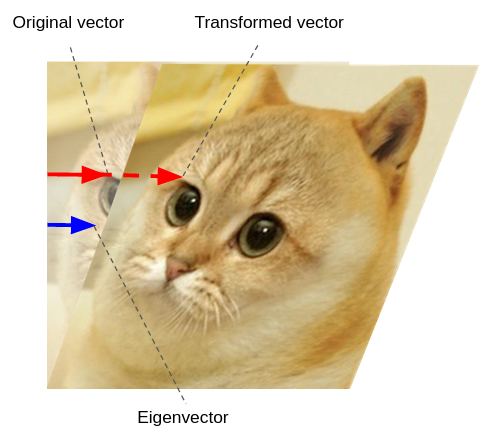
\includegraphics[width=6.5cm]{eigen-cate-sheered.png}	
\end{center}

\begin{center}
	\textbf{Figure 1}
\end{center}

\end {document}